\documentclass{article}
\usepackage{graphicx}
\usepackage{subcaption}
\usepackage{hyperref}

\title{ECNS 460 Visualization}
\author{Quinlin Gregg}
\date{November 7, 2024}

\begin{document}

\maketitle

I pulled data on touchdowns, field goals, and punts by team and season from
\href{https://www.pro-football-reference.com}{Pro Football Reference}. The code for this
is in the \texttt{/fetch} directory. This was combined with data on Australian betting odds
for NFL games. (Australia has had legalized sports gambling longer than the United States,
so their data goes farther back.)

First, datasets containing offensive and defensive statistics for various teams were merged based on common identifiers such as team and season while adding prefixed to mark whether the data was for the offense or the defense. This resulted in a single dataset that combined different types of data into a single, comprehensive record for each team.

Subsequent transformations were applied to certain variables to make them suitable for analysis. Categorical variables, such as overtime, playoff, and neutral, were converted into logical values (TRUE/FALSE). Date-based transformations were performed to get the season for each game to enable the aggregation of team performance over time. Aggregation techniques were used to calculate metrics like wins, losses, and performance against the spread, which were summarized by team and season. These aggregated statistics offered a more comprehensive view of team performance and enabled detailed comparisons across teams and seasons. Rigorous consistency checks were implemented to ensure that the number of games played and other key metrics aligned with expectations and to ensure that there was not any data lost during these transformations.

As part of the processing, I added variables for detrended and ranked touchdowns,
field goals, and punts. The reason is that, as the plots below show, all three have 
statistically significant trends over the time frame. Having two different methods of 
detrending the data should make it easier to make conclusions across seasons.

I also added per-game values for touchdowns, field goals, and punts, as well as for their
detrended versions. This is because the NFL switched from a 16-game schedule to a 17-game one 
midway through the data, so this removed the number of games in the season as a factor.

These figures show that the league is not consistent from year to year, which highlights the 
potential importance of detrending the data for better analysis across years.

\begin{figure}[ht]
    \centering
    \begin{subfigure}{0.32\textwidth}
        \centering
        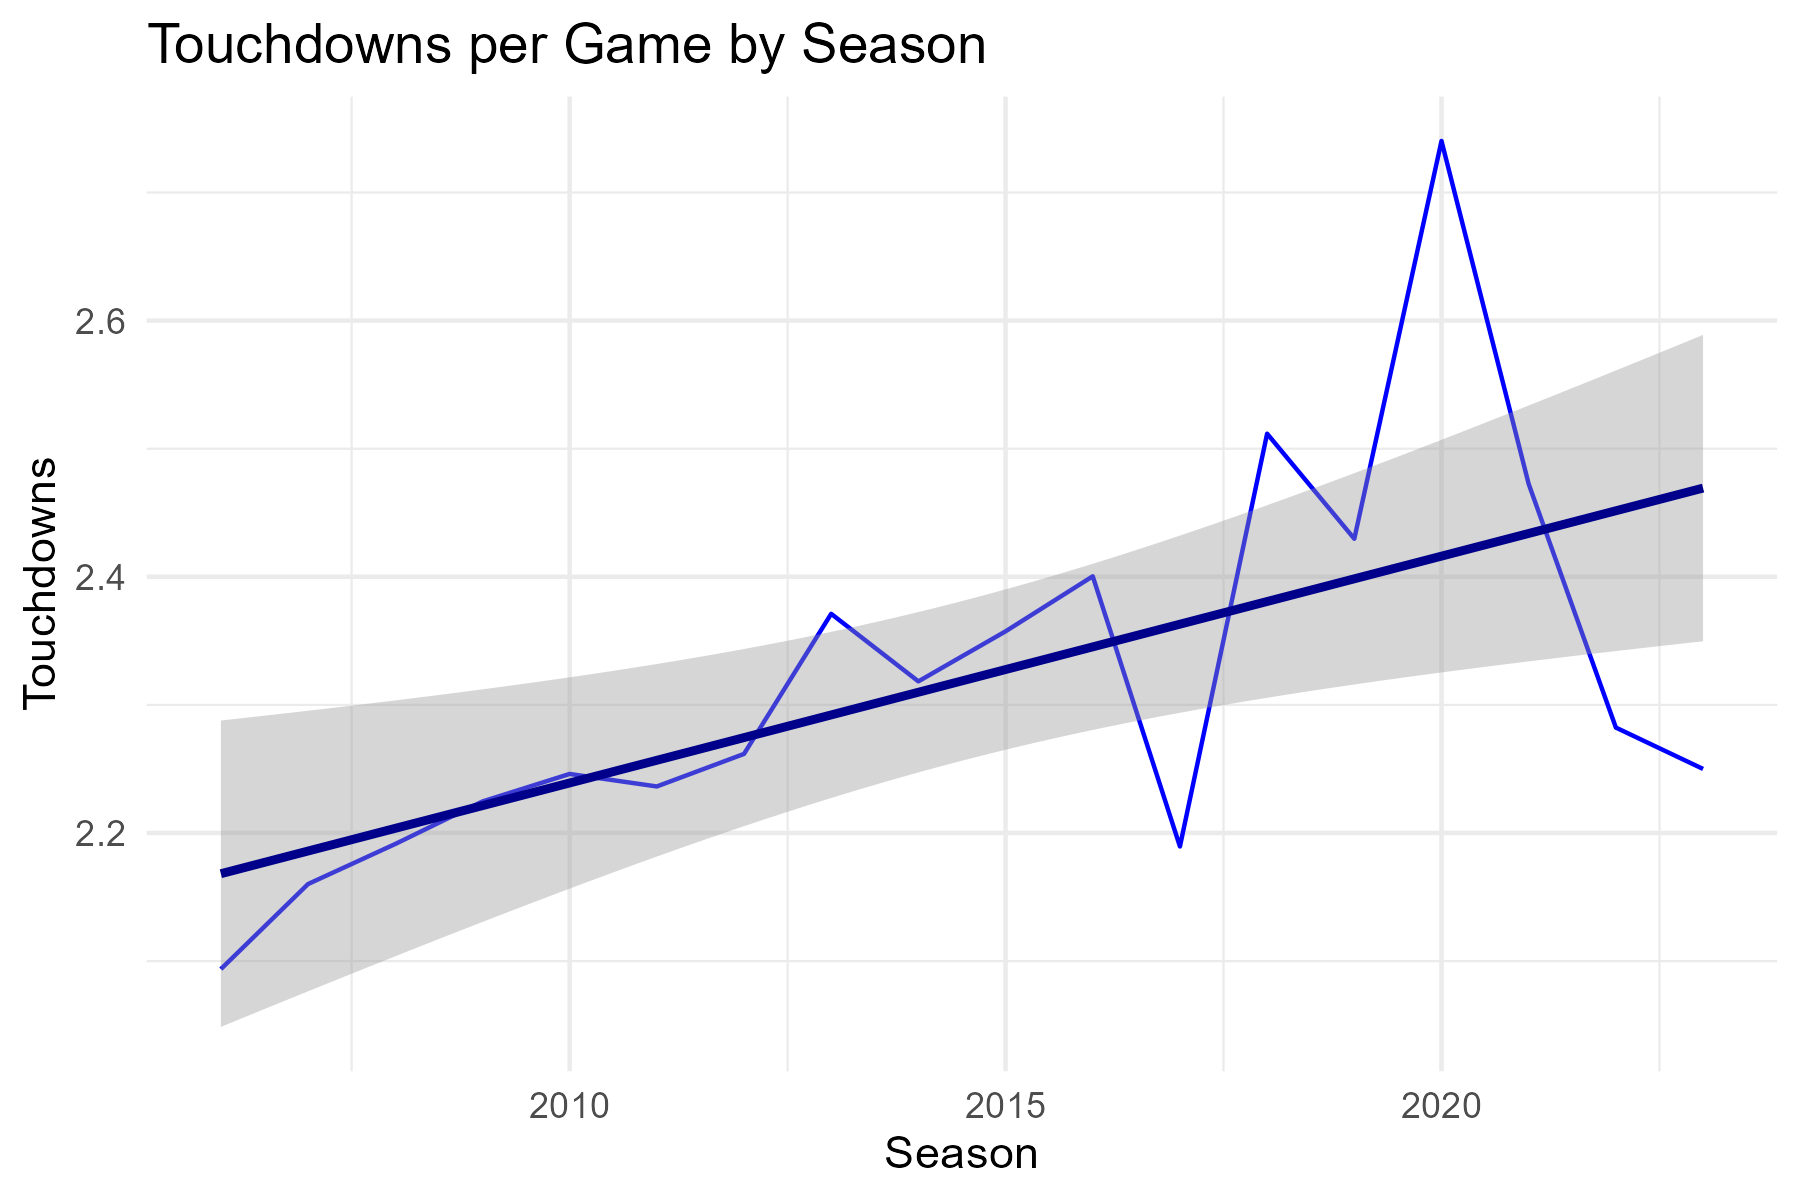
\includegraphics[width=\textwidth]{../plots/td_per_game.png}
    \end{subfigure}\hfill
    \begin{subfigure}{0.32\textwidth}
        \centering
        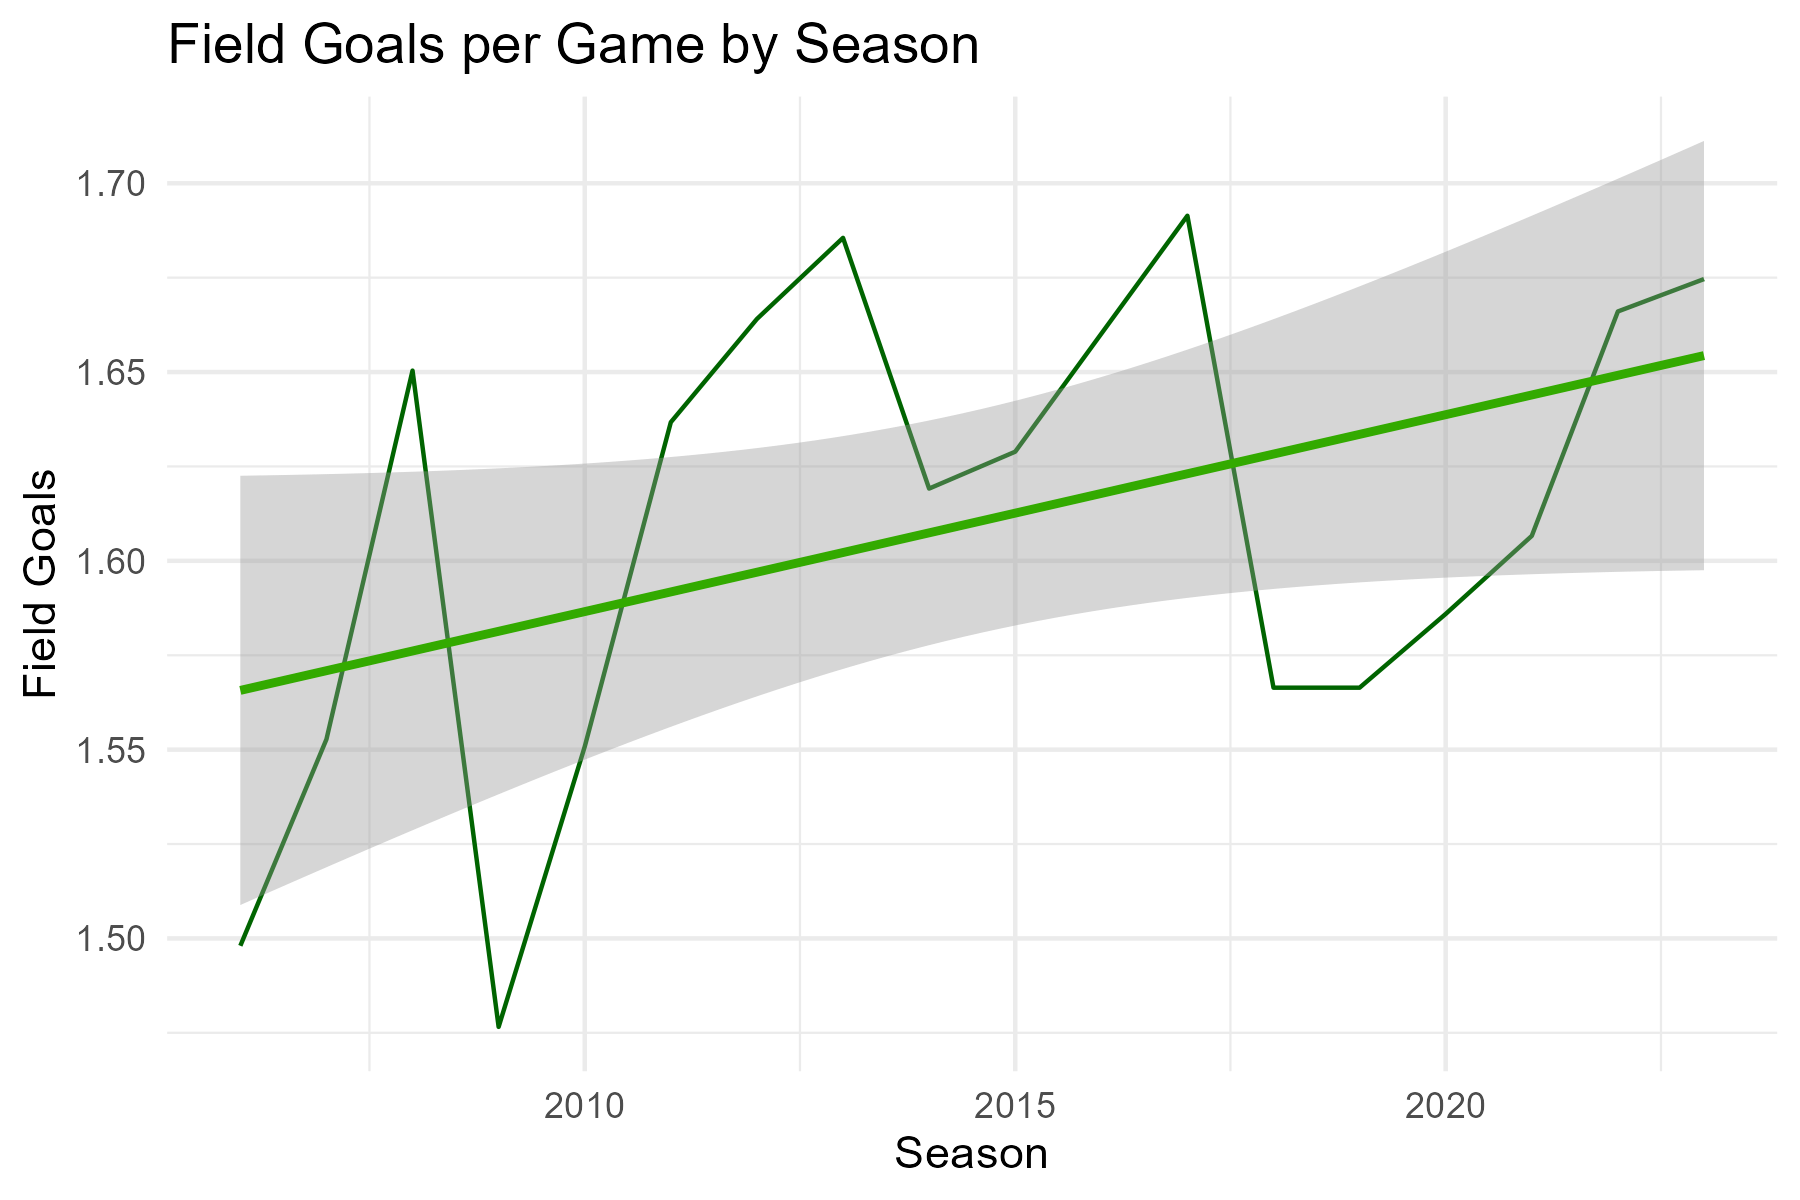
\includegraphics[width=\textwidth]{../plots/fg_per_game.png}
    \end{subfigure}\hfill
    \begin{subfigure}{0.32\textwidth}
        \centering
        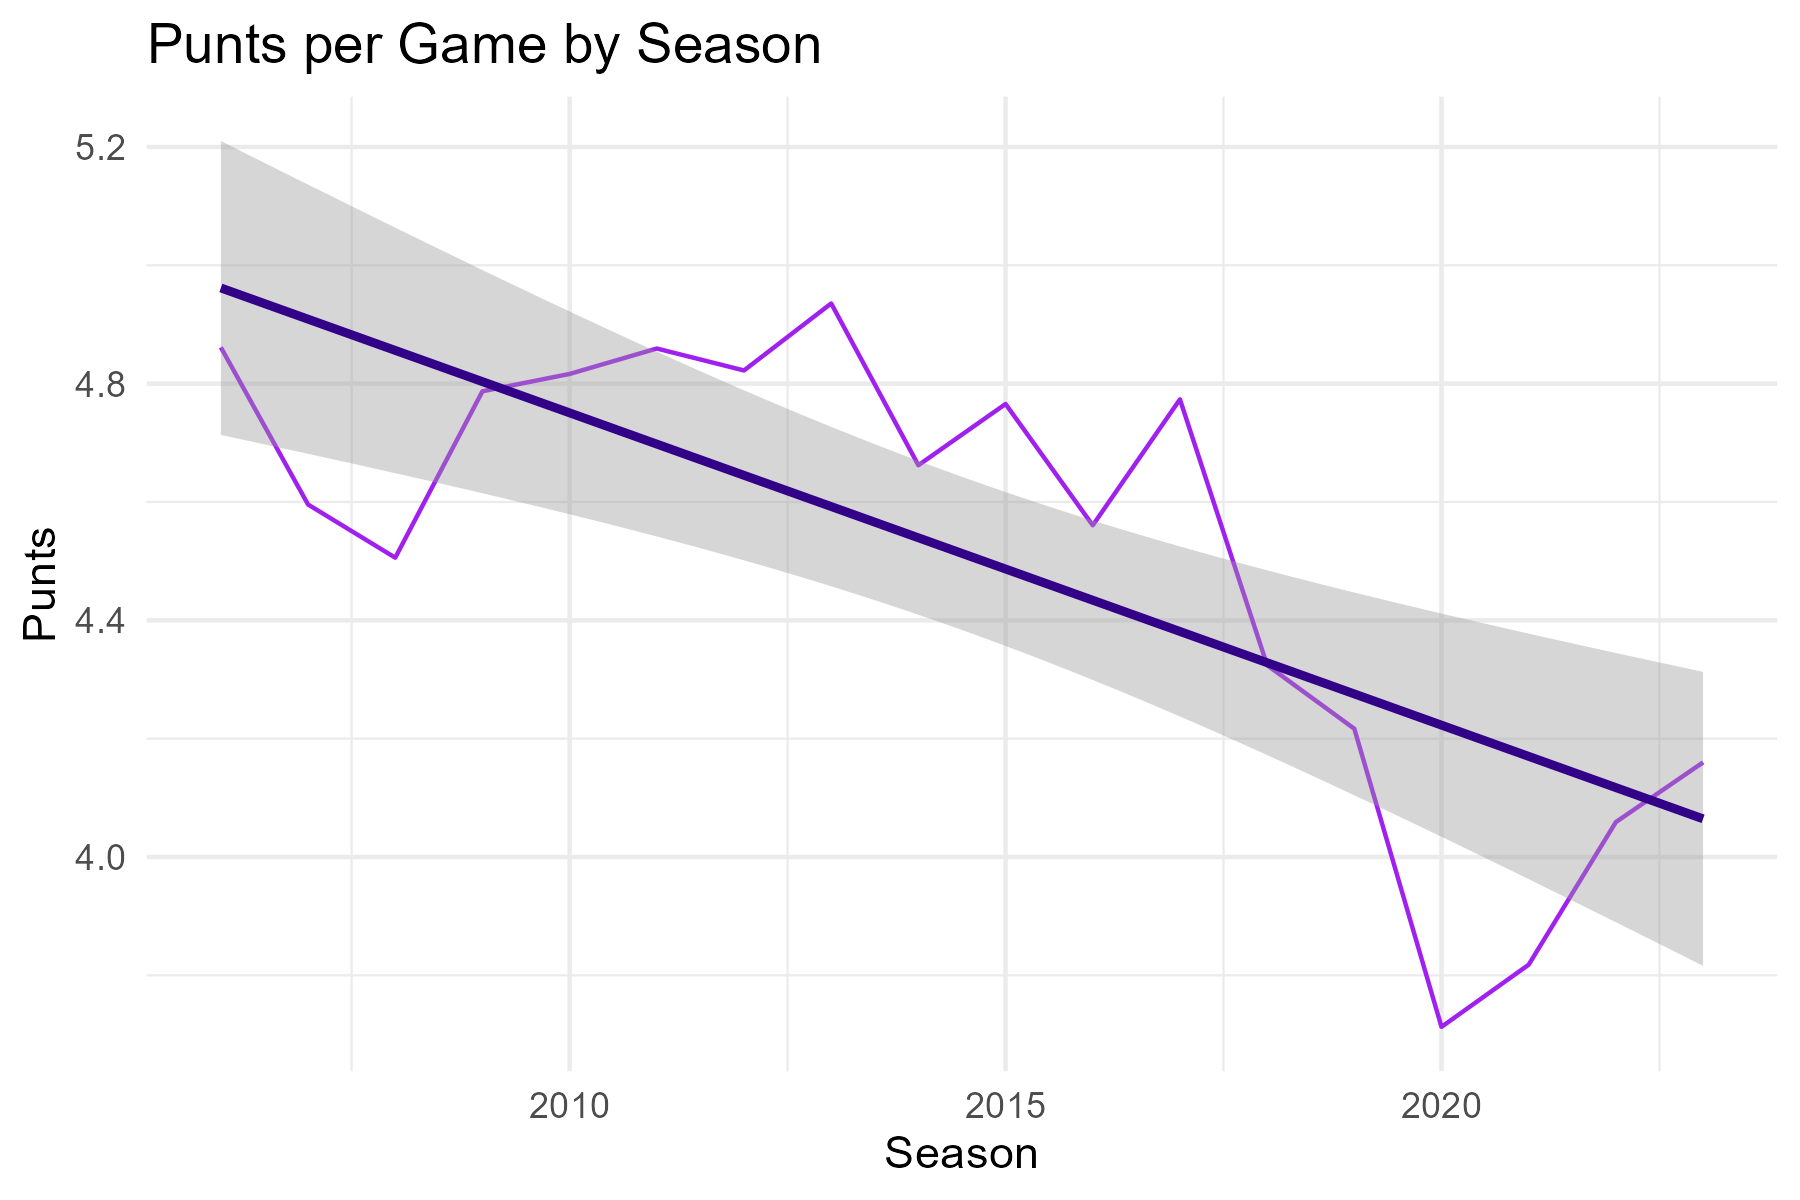
\includegraphics[width=\textwidth]{../plots/punt_per_game.png}
    \end{subfigure}
    \caption{The league-wide trends for touchdowns, field goals, and punts}
\end{figure}

Figure 2 is a plot of each team's regular season record
versus their record Against the Spread (ATS).
The larger and darker bubbles indicate more teams and seasons at that location.
There is a negative relationship between record and record-ATS,
with the least-squares line of best fit being $record_{ats} = 0.68 - 0.38 * record$. 
However, there does not seem to be a strong linear relationship, with $R^{2}=0.396$.

I chose to plot it like this because this shows the moderate linear relationship between the 
two variables while showing that some outcomes are more useful than others. The bubbles work 
especially well because the data is discrete and not continuous (you cannot in arbitrary fractions
of games, even though ties count as half of a win), meaning that the bubbles group together in columns
and rows. The columns and rows could be more pronounced if the NFL had not switched to a 17-game schedule,
as the mix of schedule lengths means that there are two grids stacked in the same plot.

\begin{figure}[ht]
    \centering
    \begin{subfigure}{0.7\textwidth}
        \centering
        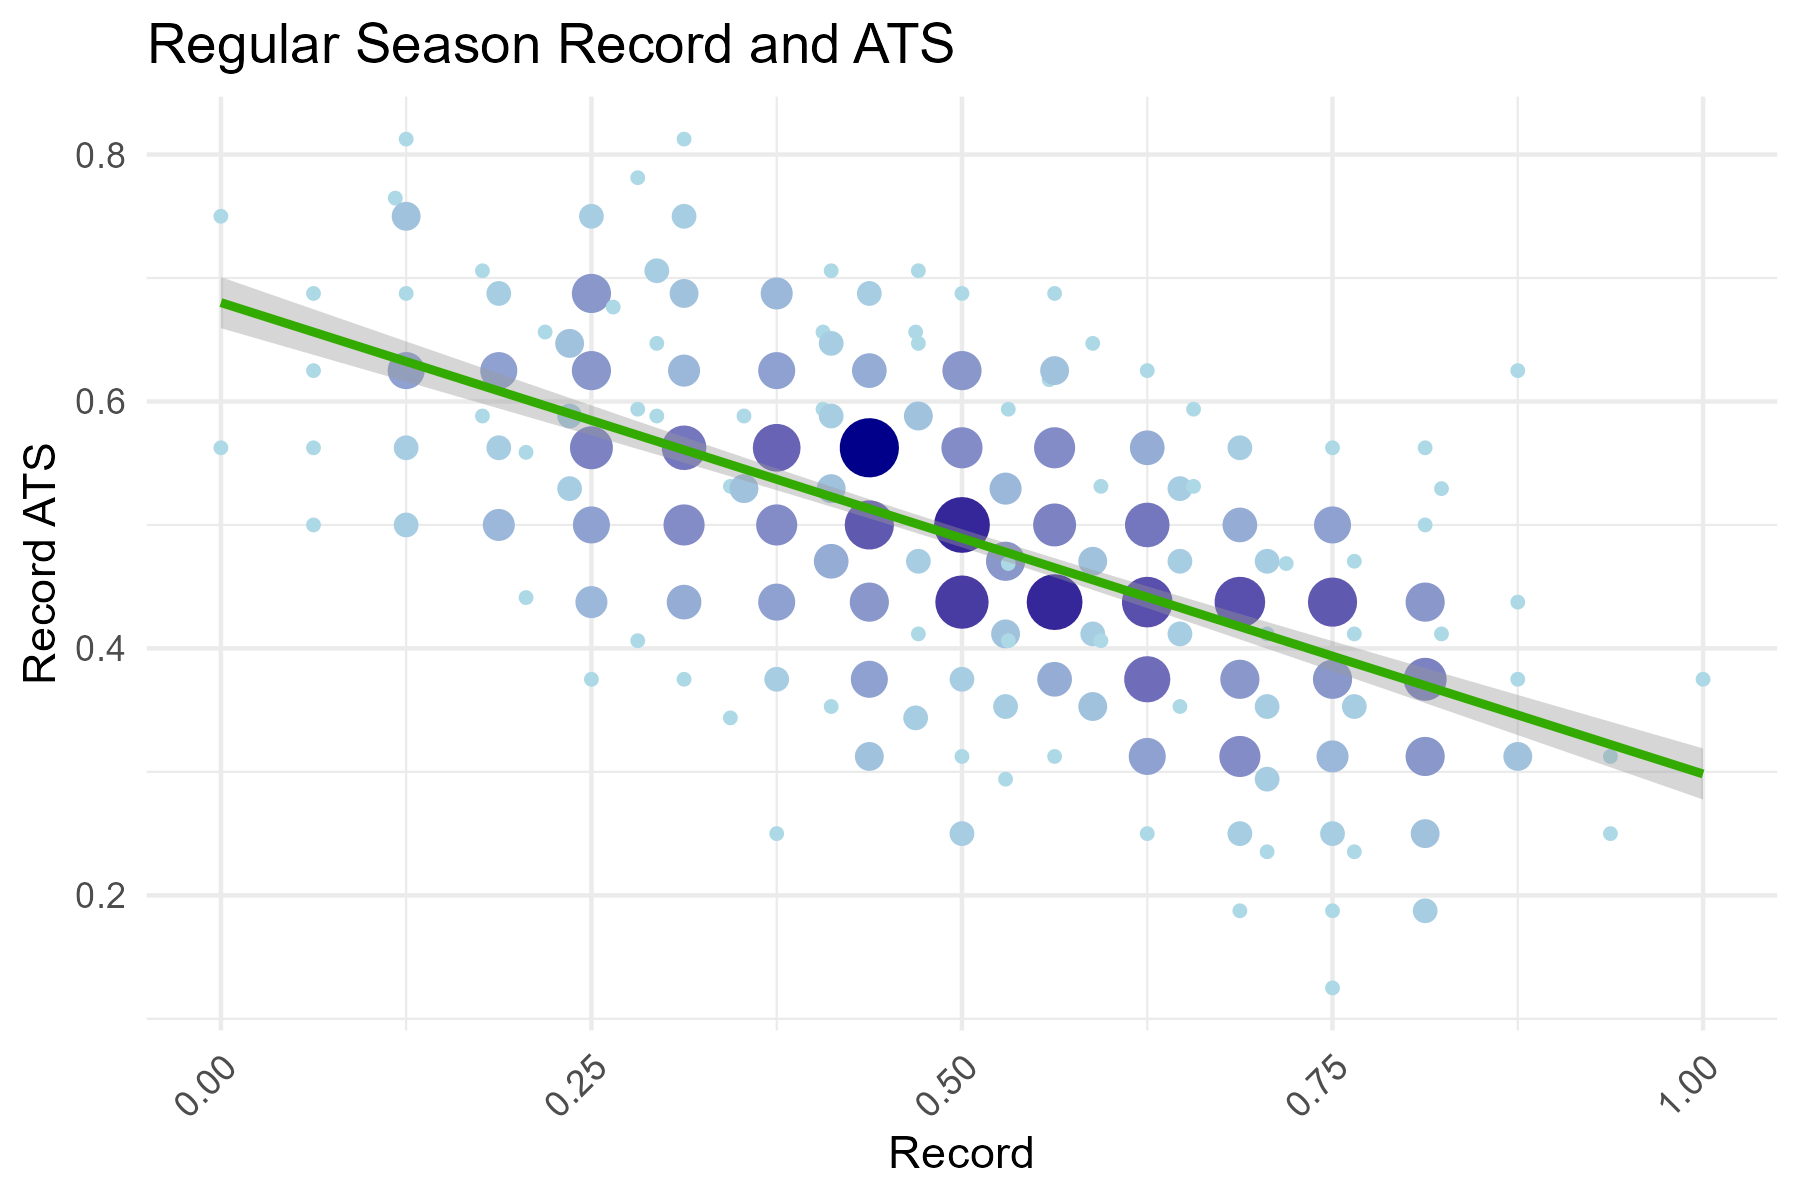
\includegraphics[width=\textwidth]{../plots/record_vs_ats.png}
    \end{subfigure}\hfill
    \caption{Each team's record versus their ATS record}
\end{figure}

I tried to visualize how consistent each team has been in this time frame.
My first measure was to take the standard deviation of each team's offensive and defense ranks
across the seasons. This produced the plot on the left, which seems to be an okay job of measuring
the "volatility" of each team until you look closer. The Kansas City Chiefs are at the far right of the 
plot, indicating a very volatile team. This is not very accurate, because the Chiefs were bad for a long time,
and then good for a long time. This is not really "volatility," but rather a team going through a single transition.
In other words, the problem with using standard deviation is that it does not understand that the data being given to
it is a time series, and so it does not respect trends. To fix this, I measured the absolute difference in ranks between seasons.
This measure takes into account the time-depended nature of the data and produces
a plot more in line with an intuitive understanding of what it means for a team to be inconsistent in the NFL.

I plotted this as a dot plot because it shows the relation between the offensive and defensive consistency
and colored each dot to the team's colors to make it easier to find in the plot.

\begin{figure}[ht]
    \centering
    \begin{subfigure}{0.48\textwidth}
        \centering
        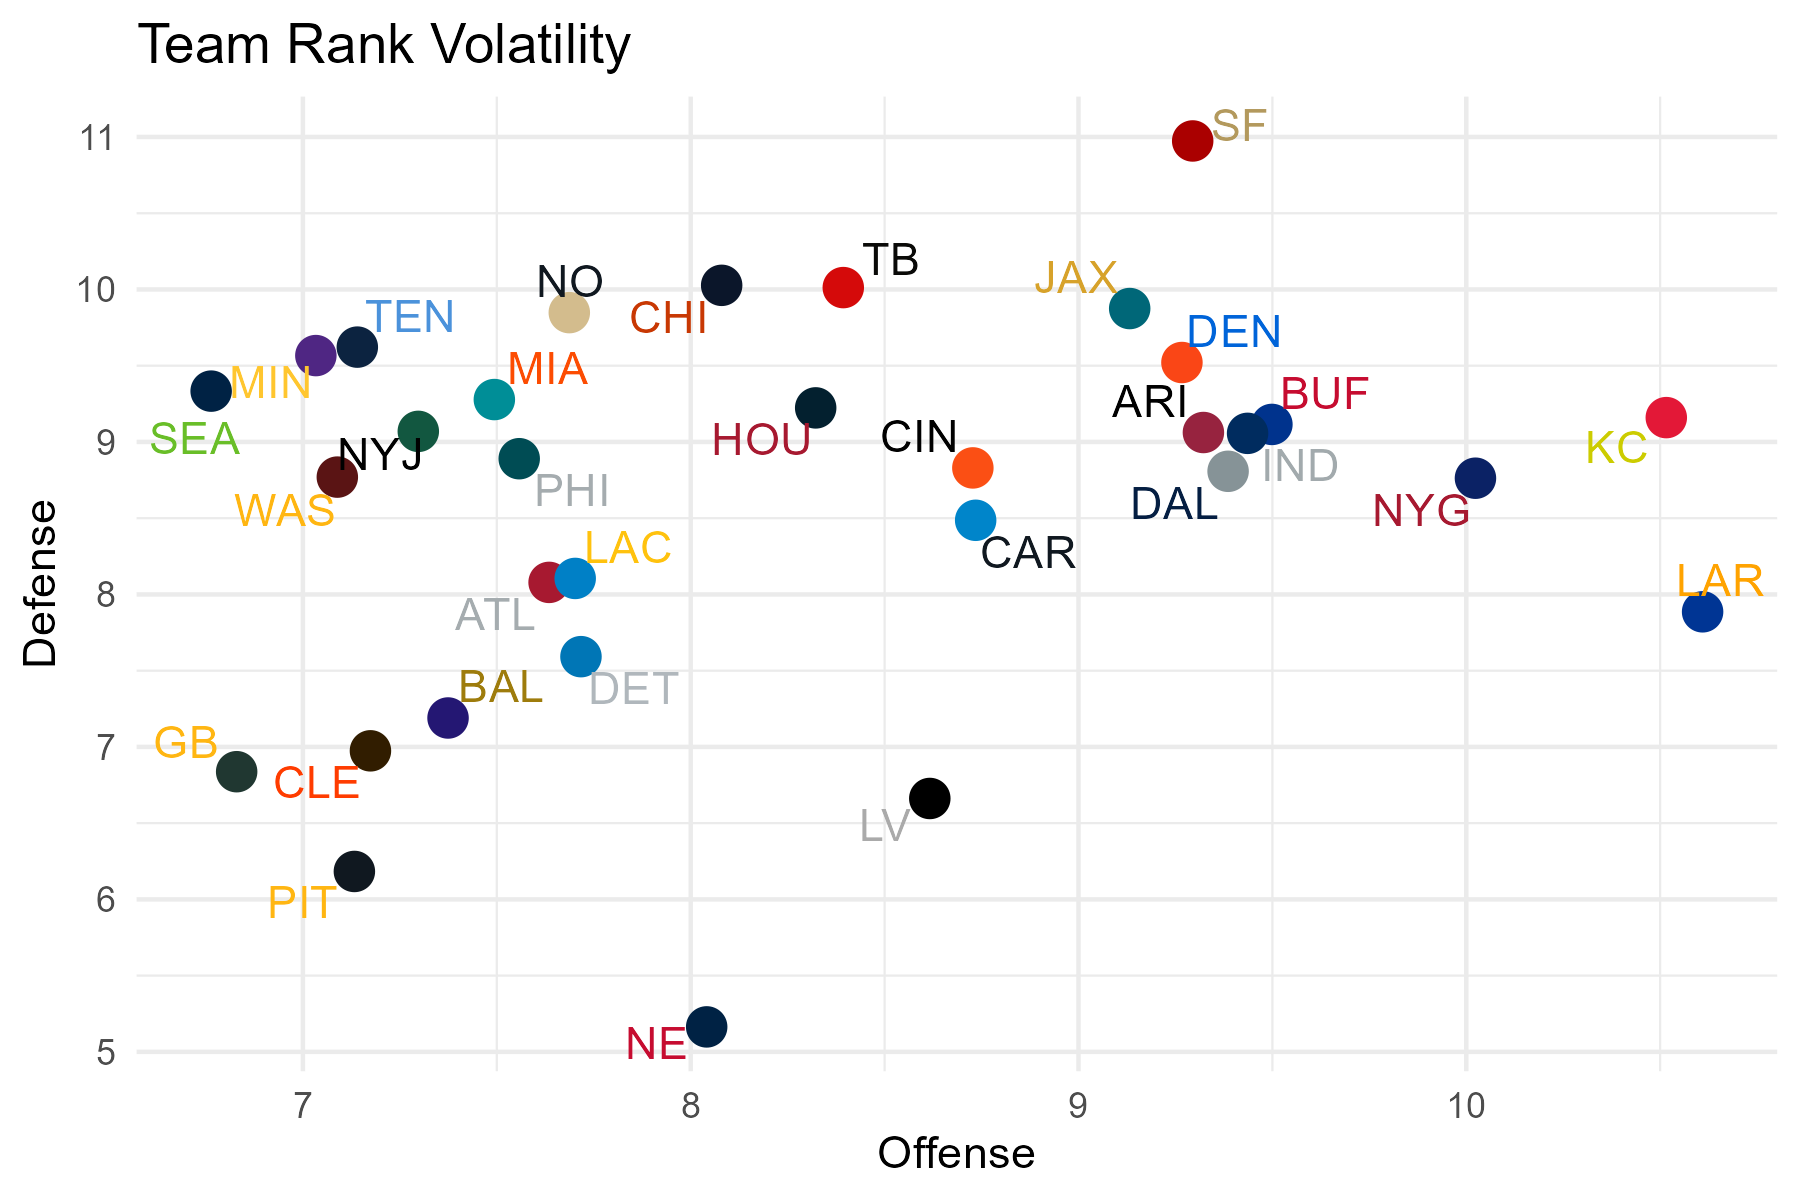
\includegraphics[width=\textwidth]{../plots/volatility.png}
    \end{subfigure}\hfill
    \begin{subfigure}{0.48\textwidth}
        \centering
        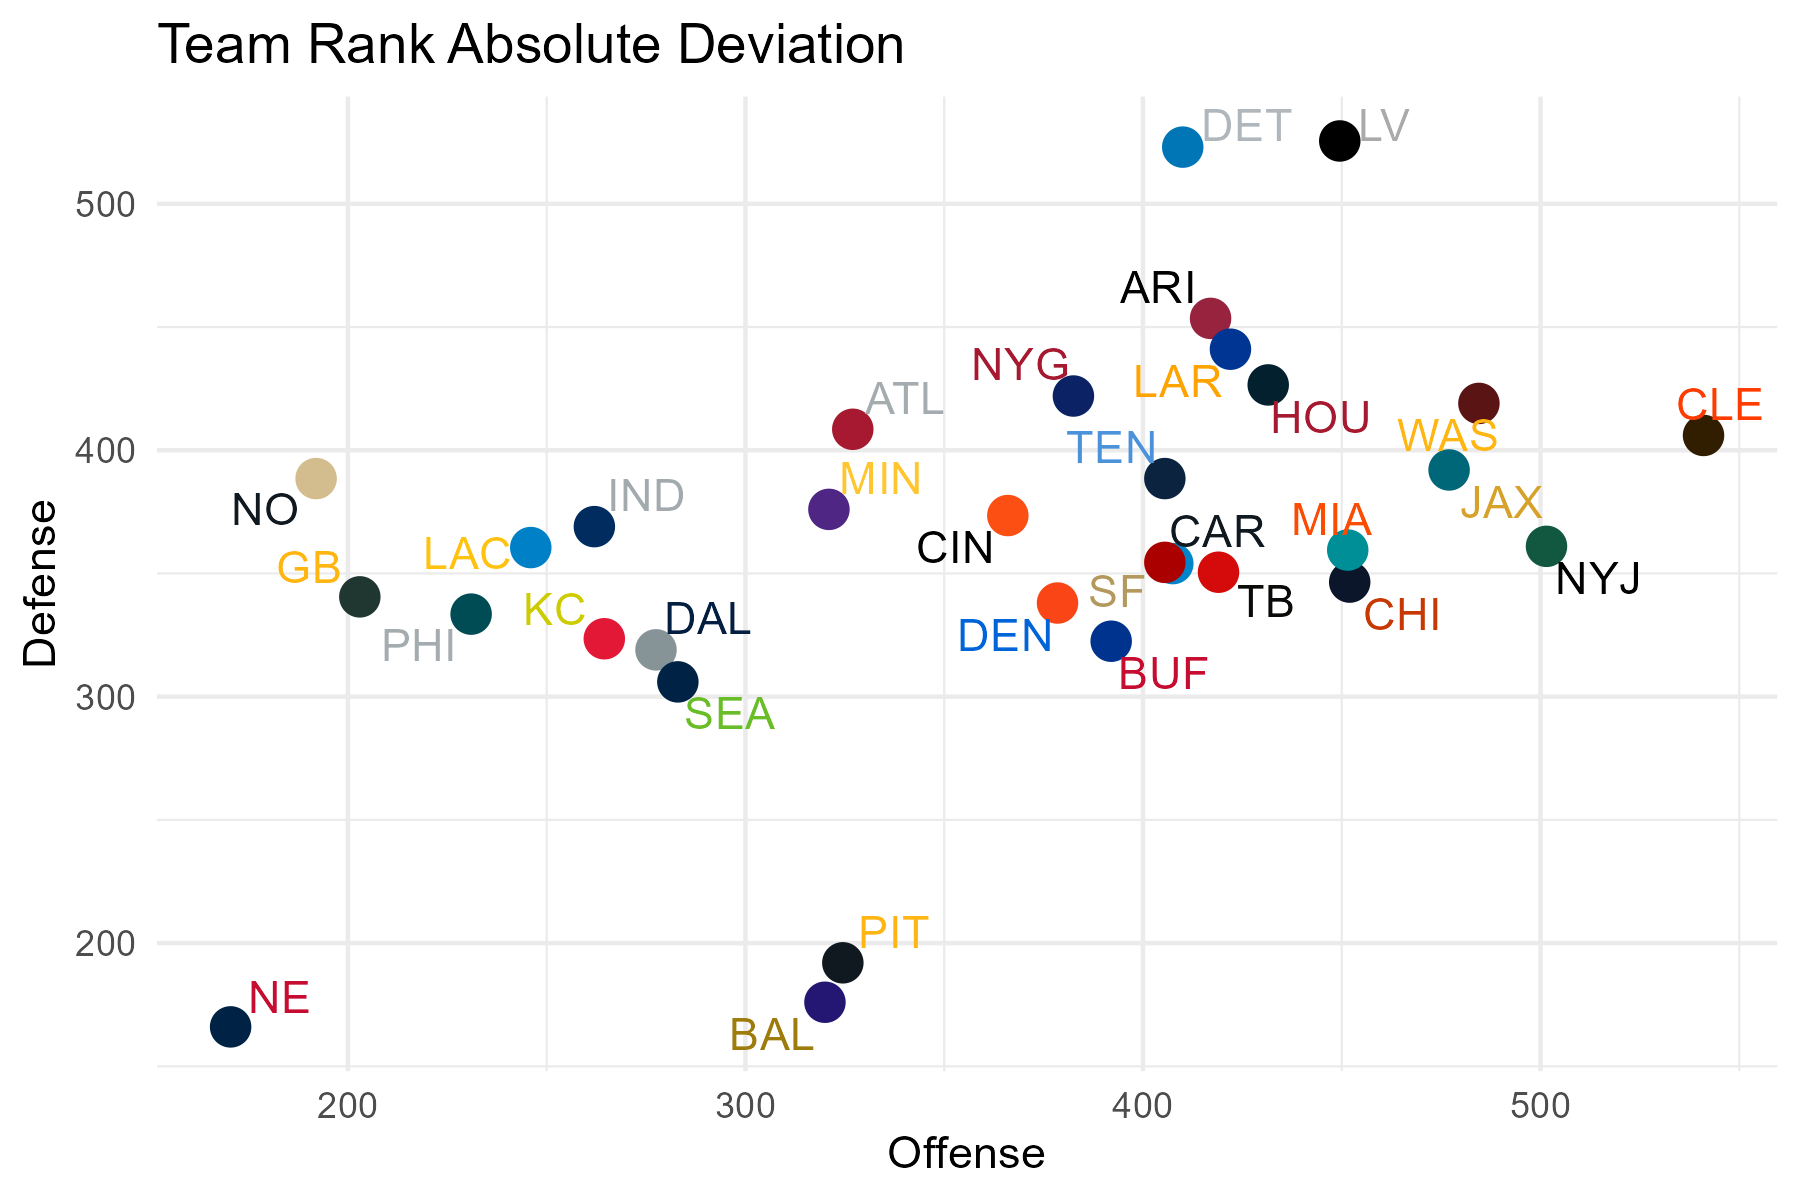
\includegraphics[width=\textwidth]{../plots/abs_dev.png}
    \end{subfigure}
    \caption{Two measures of the variance of teams' performances}
\end{figure}

\end{document}
